\section{Setting and Method}\label{classroom-study-settings}

The setting for this study was an undergraduate course in an intelligence
training program in a US university. The program was designed to train students
to become professional intelligence analysts. A key characteristic of the course is
to emphasize hands-on practice on team-based intelligence analysis.

%\bvh{do demographic stuff first}
Of the 98 students enrolled in the course (from
two sections), 73 consented to participate in the study. All of the 73 students
held major in the program of Security and Risk Analysis. Most (75\%) of them
were in the third academic year ($M=3.06 \text{ years}, SD=.44$), indicating that participants in
our study had relatively advanced experience and knowledge in intelligence
analysis. Participants' age ranged from 19 to 28 ($M=20.4, SD=1.18$). 77\% of the
participants were male.

%\bvh{I would make a bigger point about the training in the tools that they
%already had, they were sort of primed to not use a collaborative tool}

% \bvh{separate the argument about waterfall and what students were already trained in and how it played out}
During the first ten weeks of the course students learned several analytic
techniques, including IEW, ACH, timeline analysis and network analysis, as
well as state-of-the-art tools to implement these techniques, including
Analyst's Notebook and PARC ACH. Students also practiced applying these
techniques in two hands-on projects before our study. A typical workflow started
with IEW to extract and model evidence from documents, followed by building
analytic artifacts such as an ACH Matrix in PARC ACH, and a timeline and a
network graph in Analyst's Notebook. Since data from IEW table could not be
shared or extended to other tools, students had to manually replicate data for each
different tool. Most tools they used lacked serious collaboration support
(except that some teams used Google Doc to construct an IEW table). Analysts
were unable to contribute simultaneously (an issue known as production blocking
\cite{Diehl1987a}). Students divided their work by tools: each person
picked a tool and created and analyzed an artifact with the tool on their
own. This had the consequence that findings and hypotheses be made without
integrating collective efforts and diverse knowledge. Analysts coordinated work
by manually sharing documents or graphs through email or cloud storage service
(e.g.~Dropbox), resulting in a scattered placement of results, requiring
repeated manual resynchronizing to identify redundant or missing pieces of
information, analysis of information, and analytic hypotheses. In summary, the
students in our study had learned and practiced with tools lack of support for
collaboration, and were aware of the shortcomings.

Students were given a tutorial on CAnalytics a week before the project began.
One of the authors walked through the features of CAnalytics, without enforcing
or implying any strategic use of the tool. Students then accomplished a small
case analysis at their own pace. Although students were encouraged to make full
use of CAnalytics, to ensure a naturalist environment students were always free
to employ any other tools that they believed useful.

\begin{figure} \centering
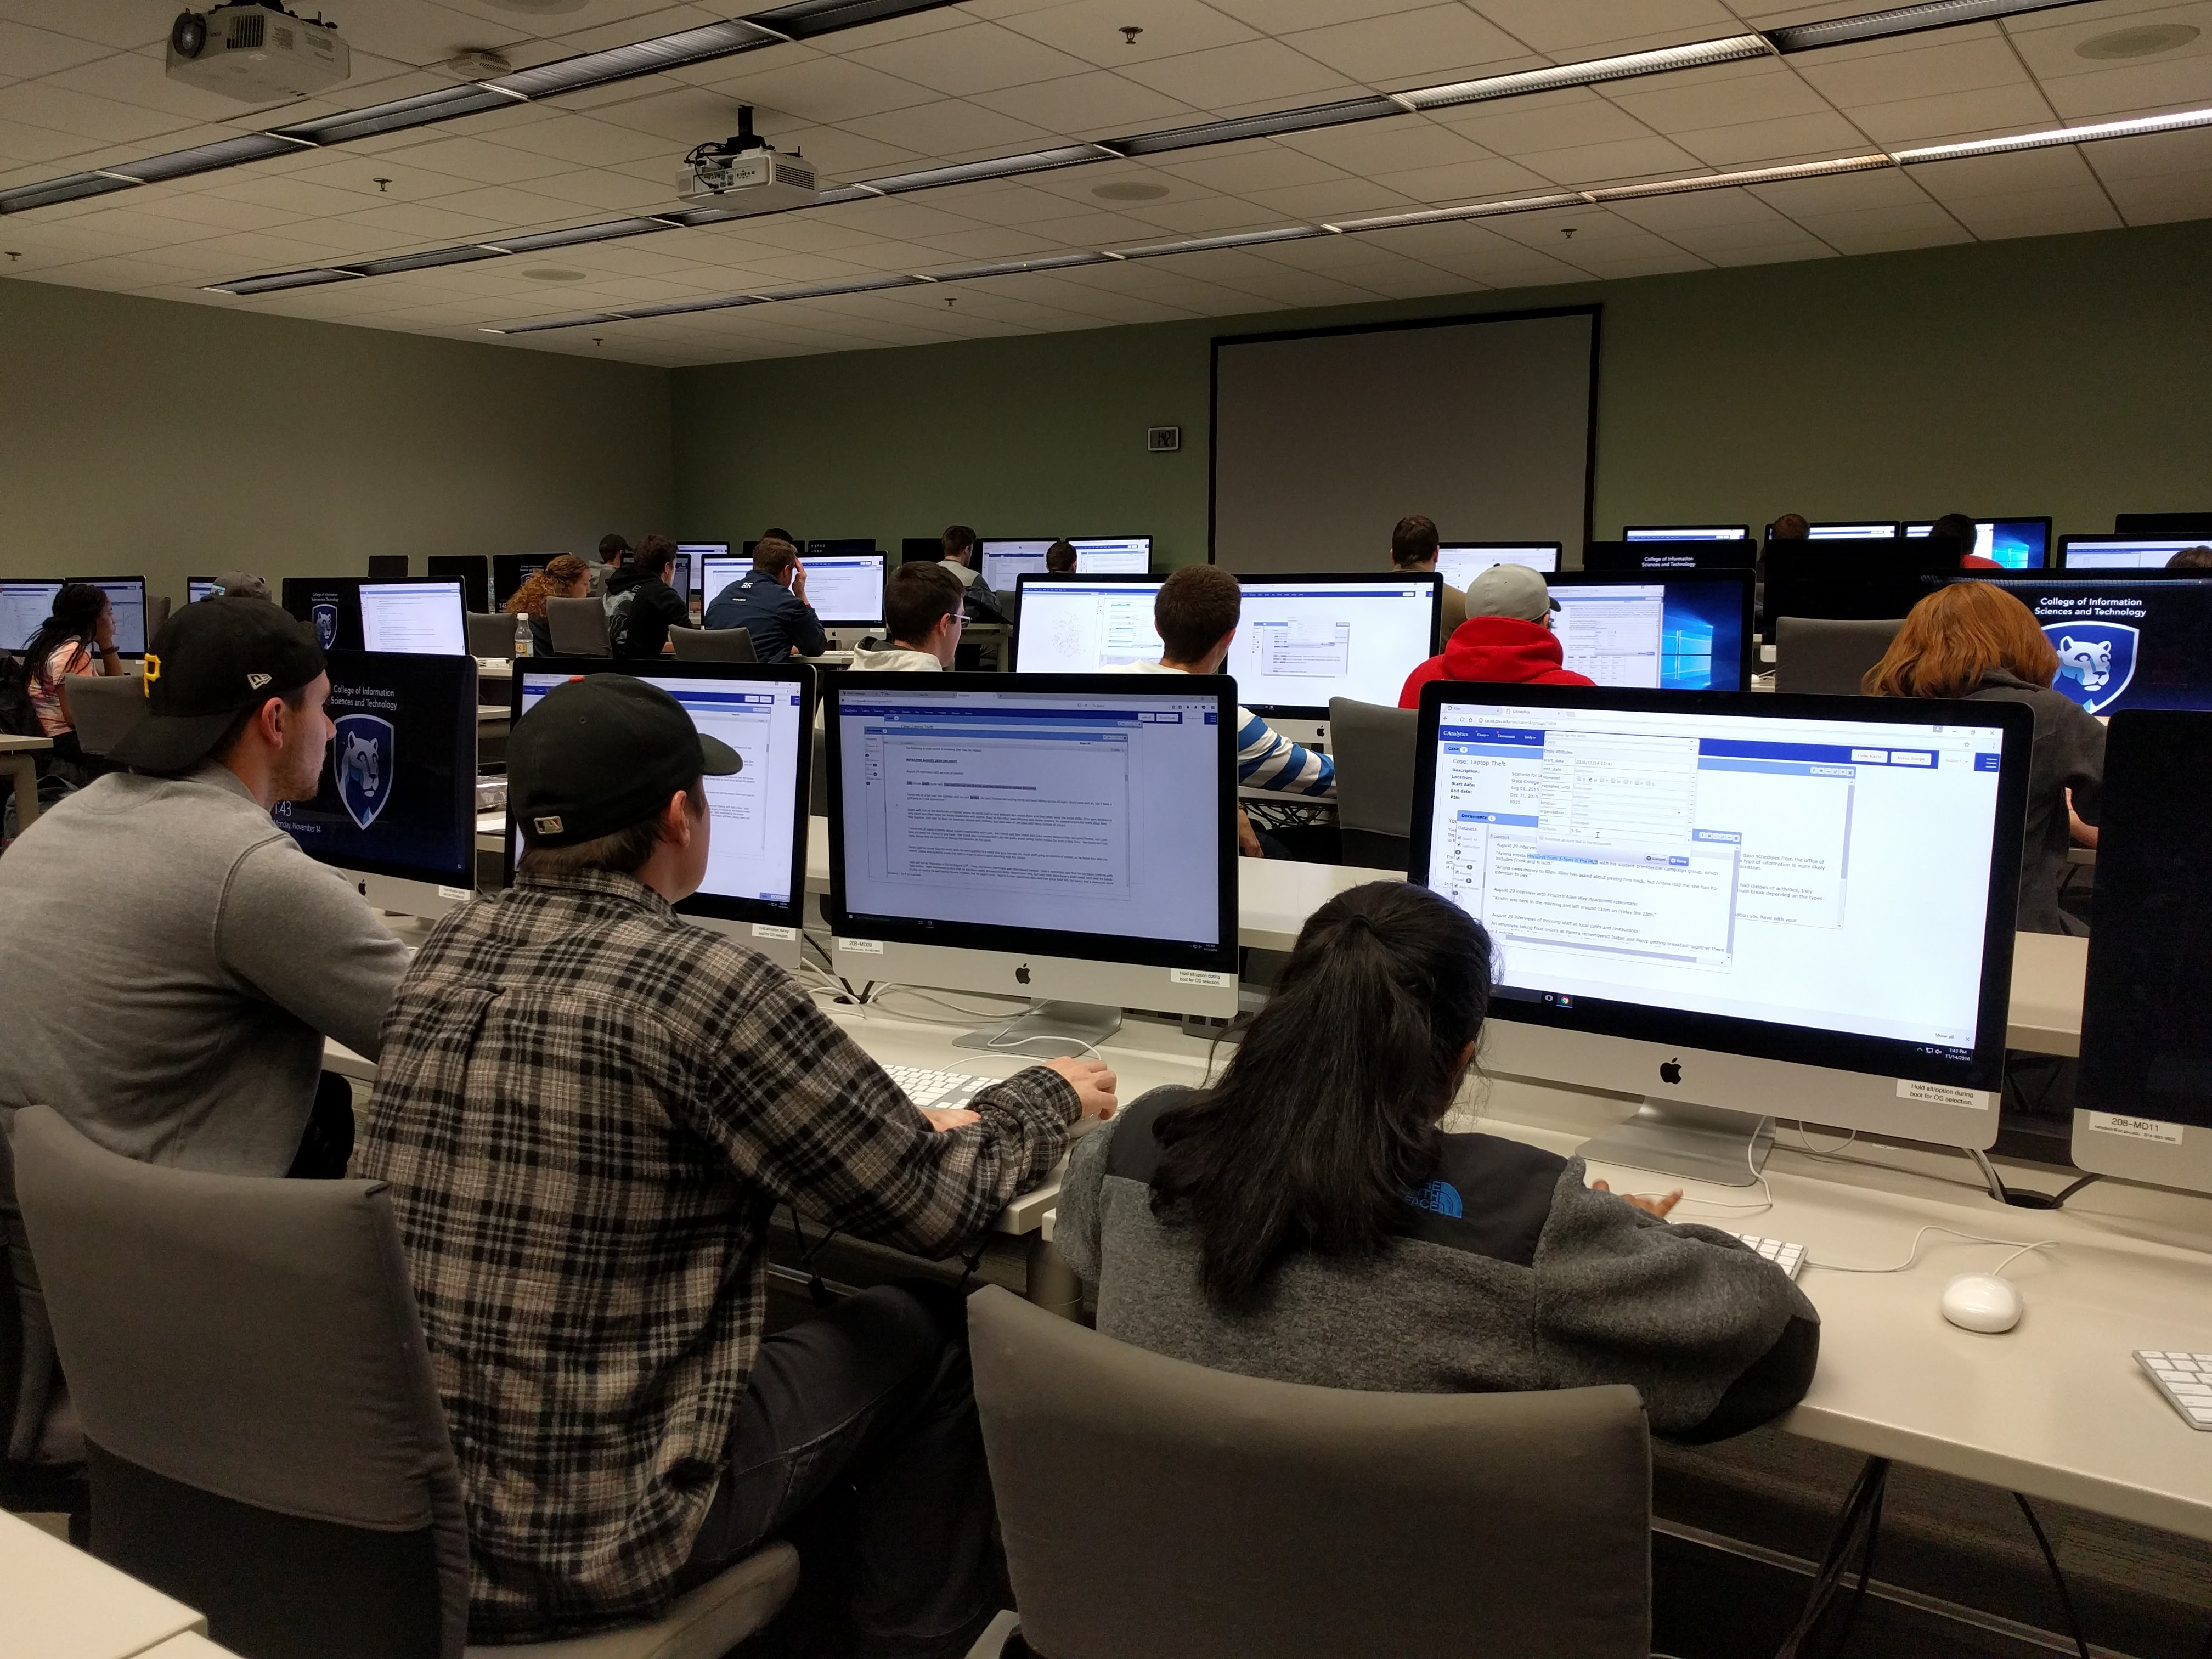
\includegraphics[width=3in]{./img/classroom_setting.jpg} \caption{Classroom
setting}\label{fig:classroom} \end{figure}

Our study began on the 10th week of the course and lasted one week. The
analysis that students performed on our tool was the investigation of
seven bank robberies fabricated by the course instructor. Teams
were provided a set of documents pertaining to the robberies, including police
reports, witnesses reports, video records, and news media. The analysis was
designed to be open-ended, meaning that there was no single, definitive answer.
The instructor explained that the task was to simulate real world scenarios, in
which analysts always reasoned in the circumstances of uncertainty, ambiguity,
and complexity. The instructor told the students that a total of 6 hours of workload was expected, including in-class and outside-class work. In the end of
the project students were required to submit a team report, describing their
hypotheses, assumptions, conclusions and supporting evidence.
Students were graded on their ability to
understand and enact the professional practices of intelligence analysis. This
strong normative emphasis on problem solving practices provides us an
appropriate evaluation context for new interactive tools: Tools are only
valuable to the students insofar as they actually support better practices and
better outcomes.

Students were randomly assigned into 25 teams (23 three-person teams and 2
two-person teams). To avoid the effect of group size on team behavior analysis, we excluded the two-person teams from our analysis in this paper. When in class, students used a 27-in Macintosh desktop. Students could use any equipment when outside class.

We employed a number of data collection approaches as suggested by prior researches \cite{Convertino2011, Goyal2016}. We administrated a post-study
questionnaire. The questions used 7-point likert scale and included nine items measuring individual's
self-reported awareness, seven items for
communication quality, six items for collective efficacy, and three items for perceived performance \cite{Convertino2011}. We also used NASA-TLX \cite{Hart1988} to measure cognitive load. The end of the questionnaire
included open-ended questions asking how the tool helped or impeded their
work. We captured user interactions with system logs. Instead of simply logging
low-level events like mouse click and keyboard strokes, we recorded actions such
as creating an annotation and deleting an entity. Finally, we reviewed team
reports and graded them as an indicator of team performance. Since the task was
open-ended, there was no single right answer. We constructed an assessment
rubric together with the course instructor by listing all possible hypotheses
and evidence from the documents, with a full score of 16. The first author and a
research assistant graded the reports independently. If the grades differ by
less than 2, an average is set as the final grade (14 out of 22 reports).
Otherwise (the rest 8 reports), the two graders review the reports together and
make an agreement.

One limitation in our classroom study is that we were unable to conduct control group comparisons. Ethically it is difficult to assign students to education conditions that may be disadvantaged. Indeed, the instructor we worked with wanted all of his students to experience the same educational opportunities. This is a direct conflict between our interest in using the classroom context as a larger-scale testbed CAnalytics, and the students/instructor interest in experiencing and learning about the effect of technology on collaborative intelligence analysis. The classroom is surely a special case of the ``real world'', but it is the real world relative to a lab study context. We often cannot run control conditions in workplaces.
